\documentclass{article}

% Language setting
% Replace `english' with e.g. `spanish' to change the document language
\usepackage[english]{babel}

% Set page size and margins
% Replace `letterpaper' with`a4paper' for UK/EU standard size
\usepackage[letterpaper,top=2cm,bottom=2cm,left=3cm,right=3cm,marginparwidth=1.75cm]{geometry}

% Useful packages
\usepackage{indentfirst}
\usepackage{amsmath}
\usepackage{graphicx}
\usepackage[colorlinks=true, allcolors=blue]{hyperref}

\usepackage{biblatex} %Imports biblatex package
\addbibresource{ref.bib} %Import the bibliography file

\title{Oil Drop Experiment}
\author{Yulong Li}

\begin{document}
\maketitle

\begin{abstract}
First performed by Millikan and Fletcher in 1913, the measurement of the charge of an electron is an important step in humanity's understanding of the atomic structure. This report discusses details on replicating Millikan's Oil Drop Experiment. First, theoretical background on how the charge carried by an oil drop can be calculated by tracking the drop's motion in the presence and absence of an electric field is provided.  Next, details on the procedure of the experiment and the collected data is discussed.Finally, steps taken to analyze the collected data is explained. The electron charge measurement in this experiment is determined to be $0.863$ e, with a standard deviation of $0.459$ e.

\end{abstract}

\section{Introduction and Motivation}
In 1897, J. J. Thompson conducted the cathode ray experiment and concluded that there exist a type of particle called electrons that reside in atoms and contain negative charges. Given this conclusion and the observed fact that an atom as a whole is charge neutral, J. J. Thompson proposed a so-called plum pudding model for atoms in 1904. In this model, Thompson envisioned the atom to be composed of two parts: a positively charged "pudding" and numerous negatively charged electrons ("plums") that are embedded in the "pudding". The charges on the "pudding" and the "plums" cancel out, resulting in an overall charge neutral atom. Although we now know that this model has various issues, it does accurately describe the negative charged nature of electrons.

Several years later in 1911, Ernest Rutherford's gold foil experiment further improved our understanding of atoms. Rutherford's experiment demonstrated that atoms have a tiny, positively charged core that Rutherford named the nucleus. The electrons, on the other hand, are not embedded in this tiny nucleus. Instead, they orbit the nucleus at a distance, much like planets orbiting the Sun (and hence the name "planetary model"). 

Given this qualitative picture of the structure of atoms, the obvious next step is to quantify this understanding. In particular, an important question that needed to be addressed is: what is the charge of a single electron? This seemingly simplistic question is in fact tricky to answer because it is challenging to pull out an electron from an atom and measure its charge individually. 

Given these background knowledge and difficulties, Robert Millikan and Harvey Fletcher designed and conducted the Oil Drop experiment in 1913 that artfully circumvents the trouble of isolating electrons but still allows for an accurate measurement of the electron charge. The remainder of this lab report is devoted to explaining the theoretical background of this experiment, how we carried it out, and the results we got from it.

\section{Theoretical Background}
\label{sec: theory}
Broadly speaking, understanding the theoretical background of the Oil Drop experiment requires two important realizations: 
\begin{itemize}
    \item As the oil drops are pumped from the atomizer and make their way through the pinhole to enter the two charged plates (a detailed explanation of the experimental setup can be found in Section~\ref{sec: setup}), some of the drops might lose some electrons and acquire an overall positive charge.
    \item Positively charged oil drops behave differently in the presence and absence of an external electric field. Quantifying this difference in behavior allows us to determine the overall charge of the oil drops.
\end{itemize}

Next, we consider the forces experienced by the oil drops in the presence and absence of an external electric field, and argue that considering this two cases together allows us to calculating the exact value of the charge of a given oil drop. \cite{columbiaManual}

\subsection{Oil Drop Falling Under Gravity Only}
An oil drop falling under gravity only (in the absence of an external electric field) experiences three forces: 
\begin{itemize}
    \item It's own weight $ mg = \frac{4}{3} \pi a_1^3 \rho_{oil} g$, where $a_1$ is the radius of the oil drop and $\rho_{oil}$ is the density of oil.
    \item The buoyant force exerted by air $\rho_{air} g V_{drop} = \frac{4}{3} \pi a_1^3 \rho_{air} g$.
    \item The retarding force at terminal velocity (according to Stoke's Law) $k v_{g}$, where $k = 6 \pi \eta a_1$, $\eta$ is the viscosity of air, and $v_g$ is the terminal velocity of the drop under gravity only.
\end{itemize}

Since the drop is moving through a viscous medium and we are analyzing its behavior at terminal velocity, these forces should balance out each other. We have:
\begin{equation} \label{eq:gravity only}
    \frac{4}{3} \pi a_1^3 \rho_{oil} g - \frac{4}{3} \pi a_1^3 \rho_{air} g - 6 \pi \eta a_1 v_g = 0
\end{equation}

Solve Equation~\ref{eq:gravity only} for $a_1$ gives us:
\begin{equation} \label{eq:a1}
    a_1 = \sqrt{\frac{9 \eta v_g}{2 (\rho_{oil} - \rho_{air}) g}}
\end{equation}

and subsequently:
\begin{equation} \label{eq:k}
    k = 18 \pi \sqrt{\frac{\eta^3 v_g}{2 (\rho_{oil} - \rho_{air}) g}}
\end{equation}

\subsection{Oil Drop Rising under Gravity and External Electric Field}
Now suppose we turn on an electric field of appropriate strength such that the oil drop begins to rise under its influence. Again since the drop is moving through a viscous medium and we are analyzing its behavior at terminal velocity, the forces on the drop should balance out. Note that since the direction of motion of the oil drop is reversed, the direction of the retarding force on it should also be reverse (now pointing downwards). Additionally, we now need to include the electric force due to the interaction of the charged oil drop with the external electric field. We have:
\begin{equation} \label{eq:gravity+E}
    \frac{4}{3} \pi {a_1}^3 \rho_{oil} g - \frac{4}{3} \pi {a_1}^3 \rho_{air} g + k v_e - n e E = 0
\end{equation}
where $k v_e$ is the retarding force as before, and $n e$ is the net charge of the oil drop, which is an integer multiple of one electron charge $e$ (the oil drop can only lose an integer number of electrons).

Note that $k$ in the retarding force is a constant, which means we can use Equation~\ref{eq:k} to substitute for $k$. Furthermore, we can also express the electric field $E$ in terms of directly measureable quantities as:
\begin{equation} \label{eq:E}
    E = \frac{V}{D}
\end{equation}
where $V$ is the voltage different between the plates, and $D$ is the distance between the plates.

Substitute Equations~\ref{eq:k} and ~\ref{eq:E} into Equation~\ref{eq:gravity+E} and solve for $n e$ yields:
\begin{equation} \label{eq:ne}
    n e = \frac{18 \pi D}{V} (v_e + v_g) \sqrt{\frac{\eta^3 v_g}{2 (\rho_{oil} - \rho_{air}) g}}
\end{equation}

\subsection{Correction}
In practice, Millikan discovered that Equation~\ref{eq:ne} is not an accurately expression for $n e$ because Stokes's Law for the retarding force fails for oil drops whose radii are comparable or smaller than the separation between air molecules. Millikan showed that a better expression to use for $n e$ that corrects for this issue is given by:
\begin{equation} \label{eq:ne corrected}
    n e = \frac{18 \pi D}{V (1 + \frac{b}{p a_1} + \frac{1}{2} (\frac{b}{p a_1})^2)^{\frac{3}{2}}} (v_e + v_g) \sqrt{\frac{\eta^3 v_g}{2 (\rho_{oil} - \rho_{air}) g}}
\end{equation}
where $p$ is the air pressure and $a_1$ is the radius of the oil drop and can be calculated from Equation~\ref{eq:a1}, and $b$ is a constant.

\subsection{Implementing the Expression for $n e$}
\label{sec:implement}
Note that Equation~\ref{eq:ne corrected} is given purely in terms of observables. In fact, all the variables are constants except for $v_e$ and $v_g$, which can be calculated by tracing an oil drop's motion between the plates. A detailed explanation of what value I used for each of the constants in my calculation can be found in Section~\ref{sec:constants}.


\section{Procedure}

\subsection{Experimental Setup}
\label{sec: setup}

\begin{figure}
	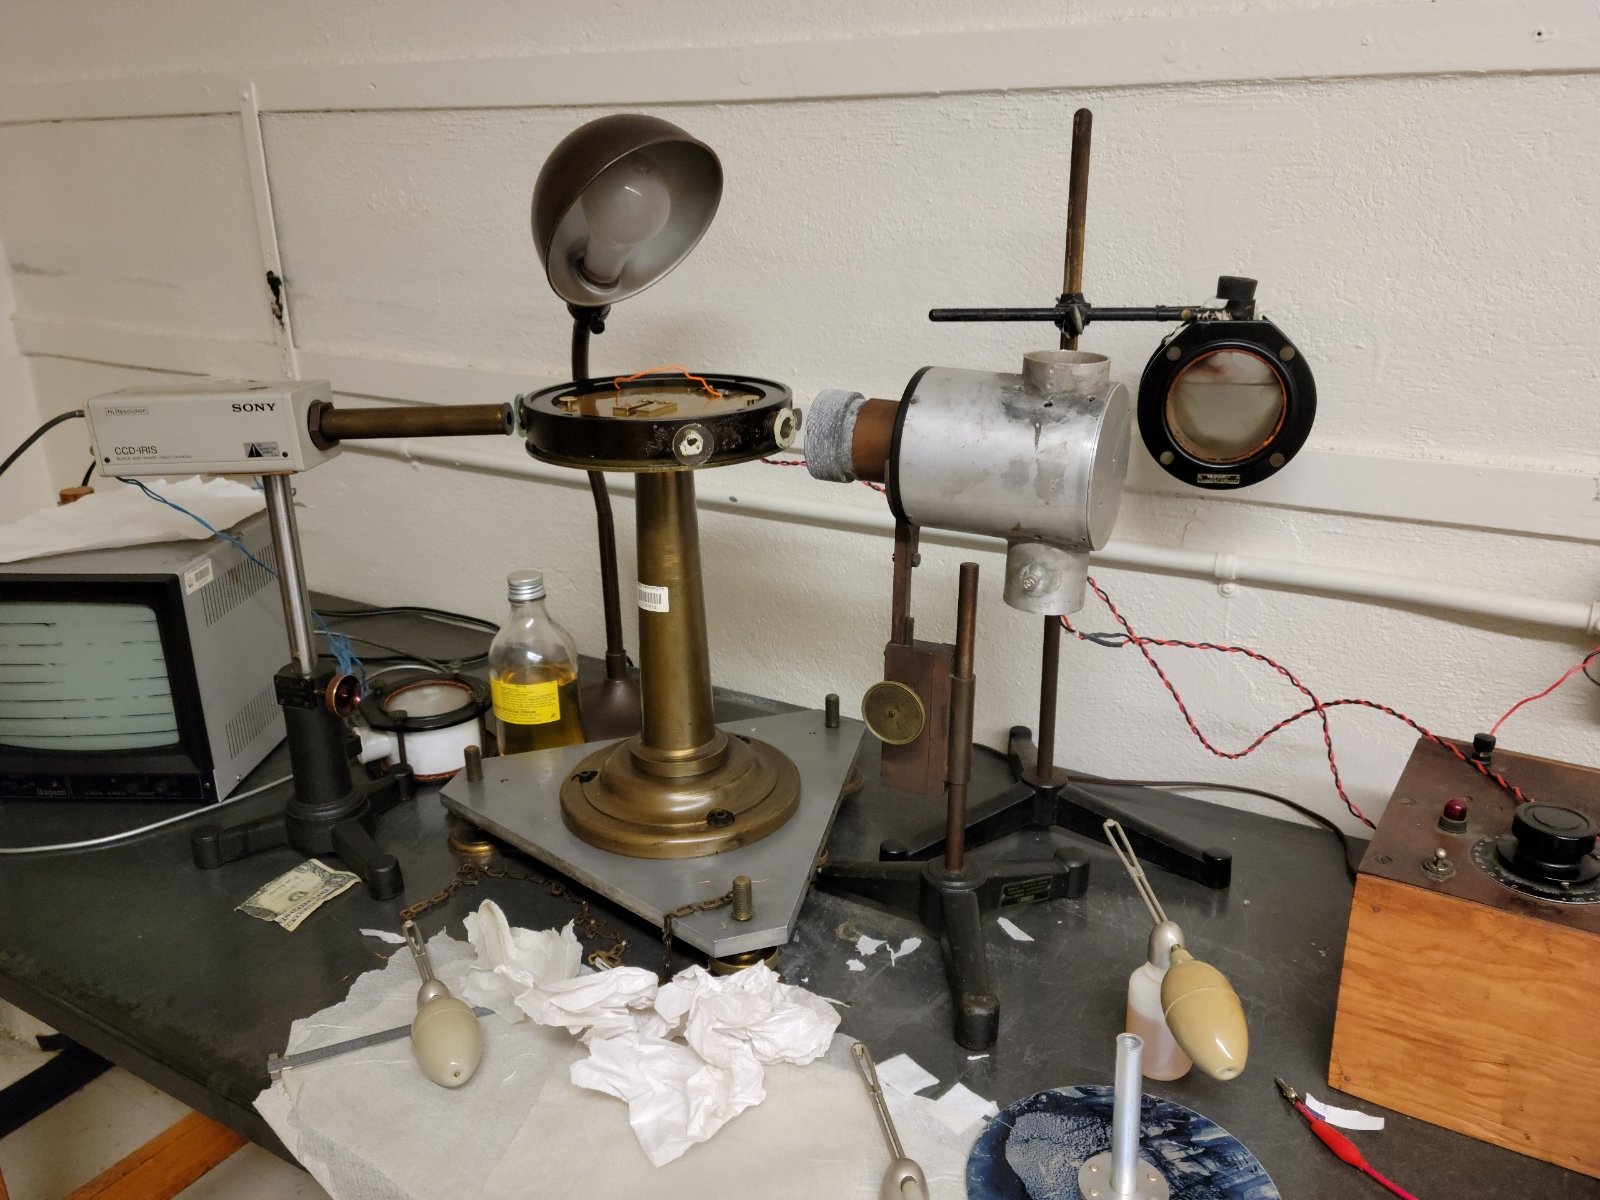
\includegraphics[width=\columnwidth]{setup.jpg}
    \caption{Setup of the experiment}
    \label{fig:setup}
\end{figure}

As shown in Figure~\ref{fig:setup}, the experimental apparatus relevant to the oil drop experiment consists of three parts:
\begin{itemize}
    \item A pair of bronze plates mounted on a stand. (shown in the middle of Figure~\ref{fig:setup}) There is a small pinhole in the middle of the top plate that allows atomized oil drops to pass through. There are apertures on the side of the mount that allows the region between the plates to be illuminated and photographed. While conducting the experiment, a lid is placed on top of the top plate to cover up the pinhole and isolate the region between the metal plates from the air current from the environment, which can affect the motion of the tiny oil drops. 
    \item A light source that serves to illuminate the region between the plates so that we can observe the motion of the oil drops. (shown on the right of Figure~\ref{fig:setup}) 
    \item A CCD camera connected to a digital screen that images the motion of the oil drops. (shown on the left of Figure~\ref{fig:setup}) 
\end{itemize}

Some other smaller parts of the experimental setup include an atomizer that pumps the oil drops, a dollar bill and a wire used for calibration, and a ruler.

\subsection{Calibrating the Apparatus}
The experimental setup mentioned above needs to be properly calibrating before it can be used to perform the oil drop experiment. A typical calibration procedure consists of three steps.
\subsubsection{Illuminate}
First, we need to ensure that the region between the metal plates is properly illuminates. Otherwise we won't be able to see the motion of the oil drops at all. To do so, we fix the position of the metal plates and adjust the height and horizontal position of the light source until its light shines exactly through the aperture and illuminates the interior of the metal plates.

Whether proper illumination is achieved can usually be judged by eye. Specifically, we simply need to remove the top metal plate and inspect the region below its original position and above the bottom metal plate to see if there is visible evidence of light shining through.
\subsubsection{Focus}
It is crucial to remember that the oil drops can only pass through a pinhole that is located at the center of the top metal plate. This implies that we not only need to illuminate the general region between the two metal plates, but also need to focus the light to the central region so that the oil drops are best resolved. This "focusing" can be calibrating in two ways.

First, we can place the top metal plate in its intended position and insert a thin wire through the pinhole. We should be able to see an image of the wire that is imaged by the CCD camera and shown on the digital screen. Next, we adjust the relative position between the metal plates and the light sources until the wire is clearly resolved on the screen. Another benefit of this method of focusing is that by repeatedly inserting and removing the wire and looking at its image on the screen, we can also ensure that we are imaging the wire itself rather than its reflection. This is essential since we will need to determine the direct of motion of the oil drops when we actually conduct the experiment.

Second, we can also remove the top metal plate and place a dollar bill vertically at the center of the bottom. Again, we will see an image of the dollar bill on the screen, and the goal is to adjust the relative position between the metal plates and the light sources until the dollar bill is clearly resolved on the screen. The advantage of this approach is that the dollar bill contains many fine-grained details on its surface. Thus, it is easier to make judgements on the focus by looking at the image of the dollar bill (as compared to the wire). 

In practice, both approaches mentioned above are perform iteratively until ideal focusing condition is achieved.

\subsubsection{Measure}
Remember in Section~\ref{sec:implement}, we discussed that the main quantities that need to be measured in the oil drop experiment are $v_e$ and $v_g$, the terminal velocities of an oil drop in the presence and absence of an external electric field. To measure these velocities, we need to keep track of the time needed for an oil drop to travel a given distance. Time can be easily measured by a stopwatch, but the measurement of distance is more tricky since we are looking at the motion of the oil drops indirectly from the image of the CCD camera, which is clearly magnified. 

To simplify the measurement of distance, the digital screen from which we are viewing the motion of the oil drops is divided into horizontal segments by black lines. If we are able to determine the physical distance between the black lines on the screen, we can simply measure the time needed for a drop to travel between adjacent black lines on the screen and deduce a velocity trivially. We refer to the distance between two black lines as the length of one division, and the lengeth of three divisions is given as $L = \frac{3}{64} inch = 0.12 \pm 0.01 cm$

\subsection{Performing the Experiment}
\label{sec:perform}
After the experimental apparatus is calibrated, we are ready to perform the oil drop experiment. A typical trial of experiment consists of the following steps.
\begin{itemize}
    \item Power on the light source, the CCD camera, the digital screen, and the voltage source. Set the voltage difference between the two metal plates to be "neutral" (0) to begin with.
    \item Use the atomizer to pump drops of oil through the pinhole and in between the plates.
    \item Gradually adjust the voltage difference between the two metal plates back and forth between "neutral" and "negative" until a drop that exhibits reasonable behavior with reasonable velocities is identified. (when the voltage is set to "negative", the top plate is negatively charge while the bottom plate is positively charged. Thus, the induced field exerts an upward force on the positively charged oil drops.)
    \item Adjust the voltage difference to "neutral". Now the identified oil drop should move downwards. Record the time needed for the drop to travel between three divisions on the screen.
    \item Adjust the voltage difference to "negative". Now the identified oil drop should move upwards. Record the time needed for the drop to travel bthree divisions on the screen.
    \item Repeated the above two steps for at least 2-3 times.
\end{itemize}

In a single trial of experiment, one oil drop is analyzed. In our experiment, we analyzed a total of 15 oil drops.

There are several points in the experimental procedure that are worth noting. First, when the oil drops are pumped into the plates using the atomizer, it is advantageous to pump in as few drops as possible. This is because we want to be able to unambiguously follow a single drop up and down several times, so the fewer distractions, the better. Second, it is crucial that we track the same drop up and down for several times. Since each of the oil drops can have different charges (hence $n e$ rather than just $e$ in Equation~\ref{eq:ne corrected}), tracking a single drop cannot be replaced by measuring the upward and downward velocities of an ensemble of oil drops. Furthermore, measuring $v_e$ and $v_g$ multiple times by following a drop up and down multiple times has the added benefit of reducing possible human error coming from timing inaccuracies. 

\section{Results}

\subsection{Values of Relevant Constants}
\label{sec:constants}
Before going into the data we collected, it is important to first establish the values we are using for all the physical constants that are relevant to this problem. With all the constant established, calculations can be carried out in a straightforward manner by following Equation~\ref{eq:ne corrected}. 

Note that all constants are expressed in cgs units.

\begin{itemize}
    \item Gravitational constant: $g = 980.66$ cm $s^{-2}$
    \item Density of oil: $\rho_{oil} = 0.8724 $ g $cm^{-3}$ at $10^o C$, $\rho_{oil} = 0.8606 $ g $cm^{-3}$ at $30^o C$. The density is linear with the temperature.
    \item The lengeth of three divisions: $L = \frac{3}{64} inch = 0.12 \pm 0.01 cm$
    \item Distance between the two metal plate: $D = 0.45 \pm 0.03$ cm
    \item Viscosity of air: $\eta = 1.81920 *10^{-4} g cm^{-1} s^{-1}$ at $20^o C$, and it has a temperature coefficient of $0.0494 * 10^{-5} / ^o C$
    \item Density of air: $\rho_{air} = 0.001205 $ g $cm^{-3}$ at $20^o C$, 1 ATM
    \item Air pressure: 1 ATM = 76 cm of Hg
    \item Constant in the correction term: b = .000617
     
\end{itemize}

\subsection{Summary of Data}
\label{sec:summary}

The data collected from the oil drop experiment is some time intervals, measuring the time a oil droplet takes to traverse a given distance. As discussed in Section~\ref{sec:perform}, we set this given distance to be the distance between three divisions on the screen. The data we collected is summarized in Table~\ref{tab:times}. We collected data for 17 drops, and for each drop, we repeated at least two trials. For the $i$-the trial, let $t_{g_{i}}$ represents the time taken by the drop to travel downwards in the absence of electric field and  $t_{e_{i}}$ be the time with the electric field. We then take the average of the times to obtain $t_{g}$ and $t_{e}$. Finally, we apply the theory presented in Section \ref{sec: theory} to $t_{g}$, $t_{e}$, and the relevant constants in Section \ref{sec:constants} to obtain $ne$, the charge of each drop. We presented $n$, charge divided by the electron charge, and $a_1$, the radius of the drop.

\begin{table*}
\caption{Times measured in $s$ for oil drops to travel upwards/downwards by 0.12 cm without/with electric field. $t_g$ represent time needed to travel downwards in the absence of the electric field. $t_e$ represent time need to travel upwards in the presence of the electric field. We report the voltage $V$ measured in volts, temperature T measured in $^o C$, charge $n$ measured in electron charge $e$, and radius of drops $a_1$ measured in $\mu m$.
}
\vspace{2mm}
\centering % used for centering table
\begin{tabular}{c c c c c c c c c c c c c c} % centered columns
\hline\hline %inserts double horizontal lines
Trial\# & \vline & $V$ & $T$ & $t_{g1}$ & $t_{e1}$ & $t_{g2}$ & $t_{e2}$ & $t_{g3}$ & $t_{e3}$ & $t_{g}$ & $t_{e}$ & $n$ & $a_1$\\ [0.5ex]
%heading
\hline % inserts single horizontal line
1 & \vline & 200.0 & 18.9 & 28.17 & 57.69 & 27.66 & 58.78 & 27.53 & 59.61 & 27.79 & 58.69 & 1.63 & 0.64 \\
2 & \vline & 200.0 & 18.9 & 76.84 & 6.41 & 81.43 & 4.45 & 86.47 & 6.92 & 81.58 & 5.93 & 2.84 & 0.38 \\
3 & \vline & 200.0 & 18.9 & 49.71 & 11.22 & 48.59 & 10.93 & 47.47 & 10.11 & 48.59 & 10.75 & 2.49 & 0.49 \\
4 & \vline & 200.0 & 18.9 & 44.05 & 8.34 & 46.49 & 8.29 & 42.77 & 8.47 & 44.44 & 8.37 & 3.28 & 0.51 \\
5 & \vline & 200.0 & 18.9 & 57.29 & 8.82 & 57.36 & 8.67 & 57.86 & 8.59 & 57.50 & 8.69 & 2.61 & 0.45 \\
6 & \vline & 200.0 & 18.9 & 42.17 & 12.00 & 39.64 & 11.54 & 38.92 & 12.65 & 40.24 & 12.06 & 2.65 & 0.54 \\
7 & \vline & 200.0 & 18.9 & 65.21 & 12.72 & 66.59 & 11.56 & NaN & NaN & 65.90 & 12.14 & 1.76 & 0.42 \\
8 & \vline & 200.0 & 18.9 & 49.50 & 7.11 & 48.53 & 7.05 & 49.91 & 7.18 & 49.31 & 7.11 & 3.49 & 0.48 \\
9 & \vline & 260.6 & 20.0 & 52.33 & 4.96 & 51.63 & 5.06 & 49.00 & 4.71 & 50.99 & 4.91 & 3.66 & 0.48 \\
10 & \vline & 260.6 & 20.0 & 46.32 & 5.66 & 46.93 & 5.43 & 49.20 & 5.60 & 47.48 & 5.56 & 3.44 & 0.49 \\
11 & \vline & 260.9 & 20.0 & 55.30 & 4.38 & 57.33 & 4.08 & 54.73 & 4.48 & 55.79 & 4.31 & 3.87 & 0.46 \\
12 & \vline & 260.9 & 20.0 & 63.03 & 5.48 & 58.85 & 5.53 & 64.39 & 5.56 & 62.09 & 5.52 & 2.85 & 0.43 \\
13 & \vline & 260.8 & 20.0 & 38.51 & 15.58 & 38.11 & 15.12 & 38.12 & NaN & 38.25 & 15.35 & 1.79 & 0.55 \\
14 & \vline & 260.9 & 20.0 & 65.29 & 8.48 & 65.22 & 8.36 & 66.93 & 7.95 & 65.81 & 8.26 & 1.90 & 0.42 \\
15 & \vline & 260.9 & 20.0 & 64.78 & 6.06 & 65.25 & 5.56 & 65.63 & 5.71 & 65.22 & 5.78 & 2.64 & 0.42 \\
16 & \vline & 261.0 & 20.0 & 50.83 & 12.21 & 46.16 & 11.33 & 48.07 & 11.78 & 48.35 & 11.77 & 1.79 & 0.49 \\
17 & \vline & 260.8 & 20.0 & 52.31 & 13.94 & 47.30 & 14.02 & 50.65 & 12.15 & 50.09 & 13.37 & 1.57 & 0.48 \\
		
\hline\hline %inserts single line
\end{tabular}
\label{tab:times} % is used to refer this table in the text
\end{table*}

\subsection{Uncertainty in the Results}
\label{sec:uncertainty}

\begin{figure}
	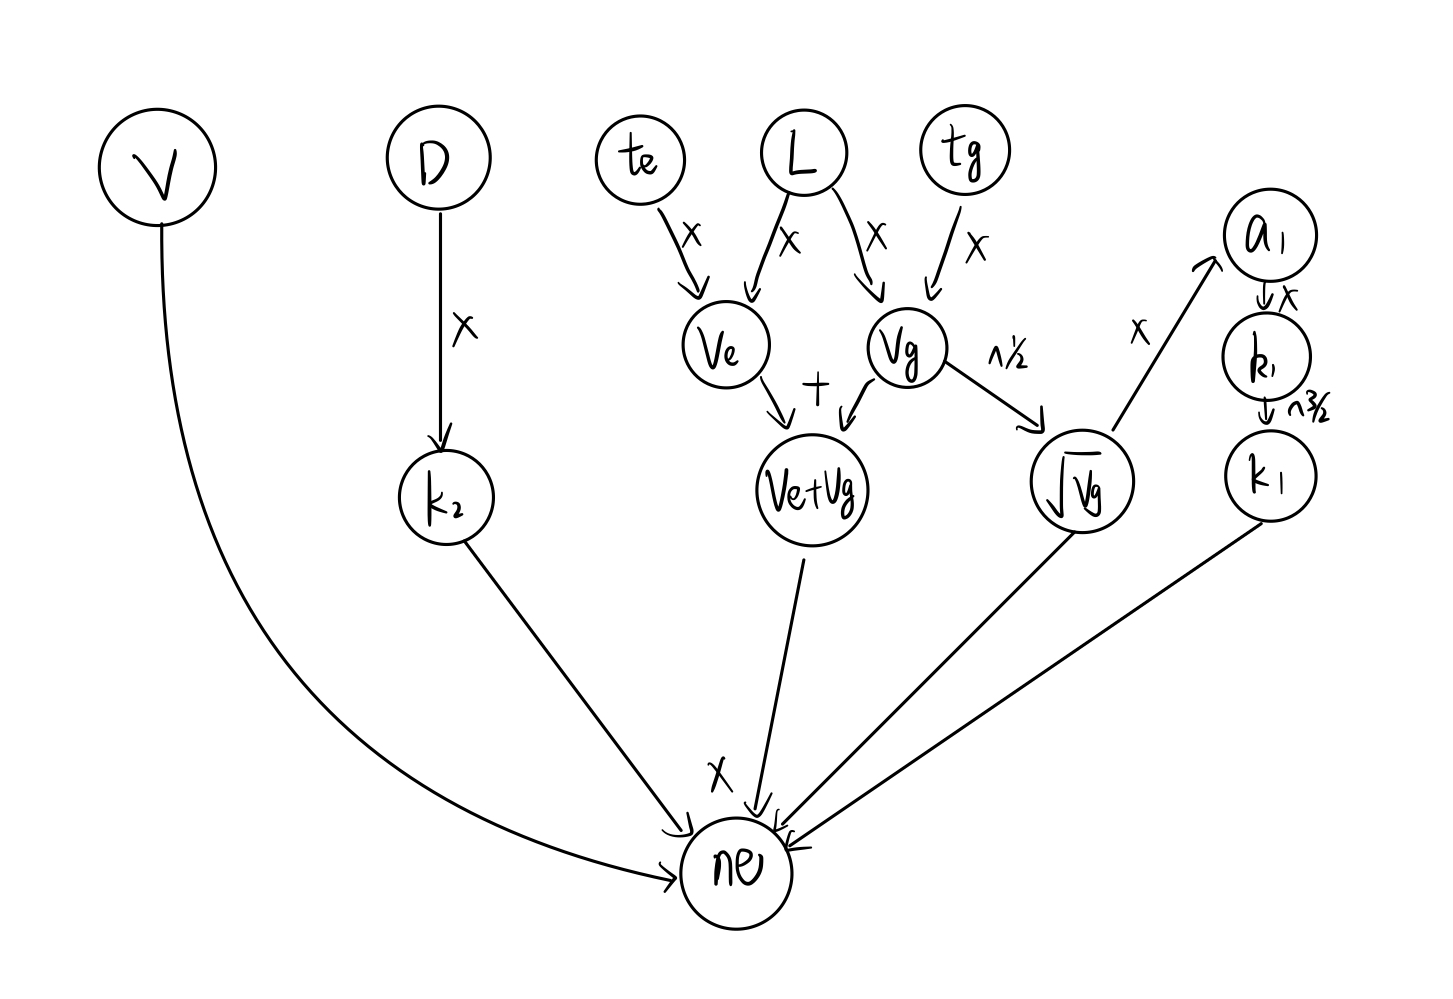
\includegraphics[width=\columnwidth]{error.jpg}
    \caption{Error Propagation in the Calculations}
    \label{fig:error}
\end{figure}

\begin{figure}[h]
	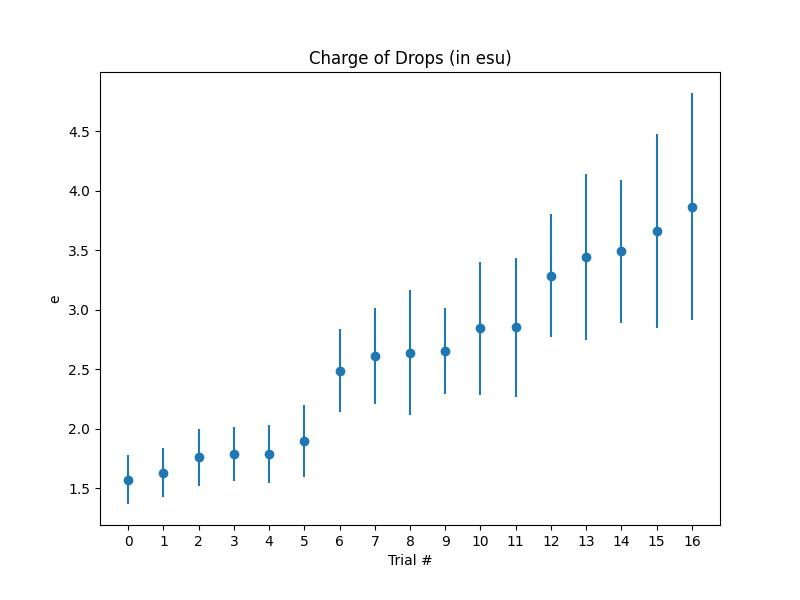
\includegraphics[width=\columnwidth]{drop_charge.jpg}
    \caption{Charge values vs. \# of drop, where the drops are ordered in increasing charge value. The charge values are measured in $e$, the electron charge.}
    \label{fig:order}
\end{figure}

\subsection{Calculation of Electron Charge: First Attempt}
\label{sec:attempt1}

\subsection{Calculation of Electron Charge: Maximum Likelihood Estimation}
\label{sec:bayesian}

\begin{figure}[h]
	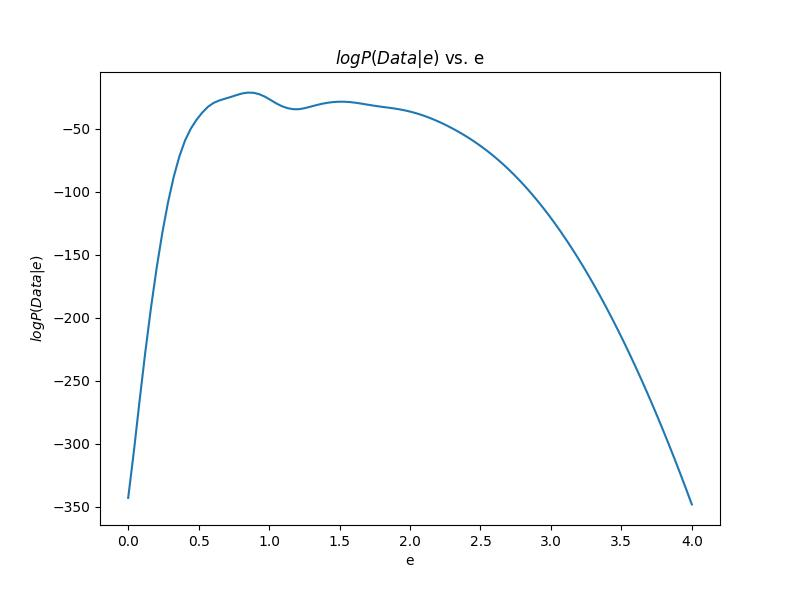
\includegraphics[width=\columnwidth]{mle.jpg}
    \caption{$log P(Data|e)$ vs. $e$, the likelihood of the observed data given a specific value for the electron charge.}
    \label{fig:mle}
\end{figure}


\section{Discussion}

\subsection{Sources of Error}
\label{sec:sources}

\subsubsection{Timing Error}
As discussed before, as we track the oil drops, we measure the time it takes for the oil drop to traverse up or down between three divisions of black lines. That is, we start timing when the oil drop hits a black line on the screen and stop timing when the oil drop hits another black line that is immediately above or below the line we started with. Multiple things can go wrong in this timing procedure. First, the black lines on the screen have some finite width, and the judgement of beginning and stopping the timer is purely made by eye. Any inaccuracies here can lead to either an overestimate or an underestimate of the time. 

\subsubsection{The Impact of Air Currents}
As discussed in Section~\ref{sec: setup}, when the experiment is conducted, a lid is placed on top of the pinhole to prevent air currents from entering the metal plates and affect the motion of the oil drops. However, this setup is not perfect, and sometimes we can clearly see the oil drops travelling in curved trajectories or trajectories that are not strictly perpendicular to the black lines on the screen. This implies that the effect of air currents is not completely taken care of. Although my partner and I have tried our best to select the oil drop that are least affect by the air currents and discard oil drops whose motion are clearly "flawed", it is still possible that the air currents affected the accuracy of our measurements.

\subsubsection{The Possible Need for More Trials}
To systematically reduce human errors in the measurements, we should to perform more trials for each drop. However, due to the time limits and the difficulty to focus on a specific drop, we are only able to complete about 3 trials for each drop.


\subsection{Code Used for Calculations}
A jupyter notebook containing the code I used to perform the calculations mentioned in this lab report can be found at this \href{https://github.com/raindragon/oil_drop}{URL}.


\printbibliography


\end{document}